%----------------------------------------------------------------------------------------
%	LAB BOOK CONTENTS
%----------------------------------------------------------------------------------------

\labday{Friday, 08 July, 2016}


%-----------------------------------------

I have been remiss in writing in the research journal.  Many things have happened.
I won't even bother trying to summarize.  Hopefully I can start to become regular
again.

\experiment{Nondiagonal Stabilization}
Digging up this old problem.  I never published it, but a good portion of the work is ready to go.
It seems that a nondiagonal stabilization parameter could be useful for MHD problems.  Assad and I
developed such a paramter for MHD and got some promising results.  I no longer have access to those
results, but I'd like to publish them.  I'm trying to use \fenics to generate the results.

At the moment, I have a Burger's implementation that solves the steady Burger's equation,
\begin{align}
 u\pdeone{u}{x} = \nu\pden{u}{x}{2}, \quad u\lr{x_{L}} = u_{L}, \ u\lr{x_{R}} = u_{R} \label{eq:burgers}
\end{align}
where the left ($u_{L}$) and right ($u_{R}$) boundary conditions are determined from
\begin{align}
  \frac{1}{2}\lr{x_{R}\lr{1-x_{*}} + x_{L}\lr{1+x_{*}}} = u_{*}
\end{align}
where $*$ can be either $L$ or $R$ indicating left or right.  Right now I am using
$x_{L} = -1$ and $x_{R} = 1$ which gives $u_{L} = -1$ and $u_{R} = 1$.  This gives
a ``shock'' at the center of the domain as shown in figure~\ref{fig:burgers_shock}.
\begin{figure}[h!]
  \centering
  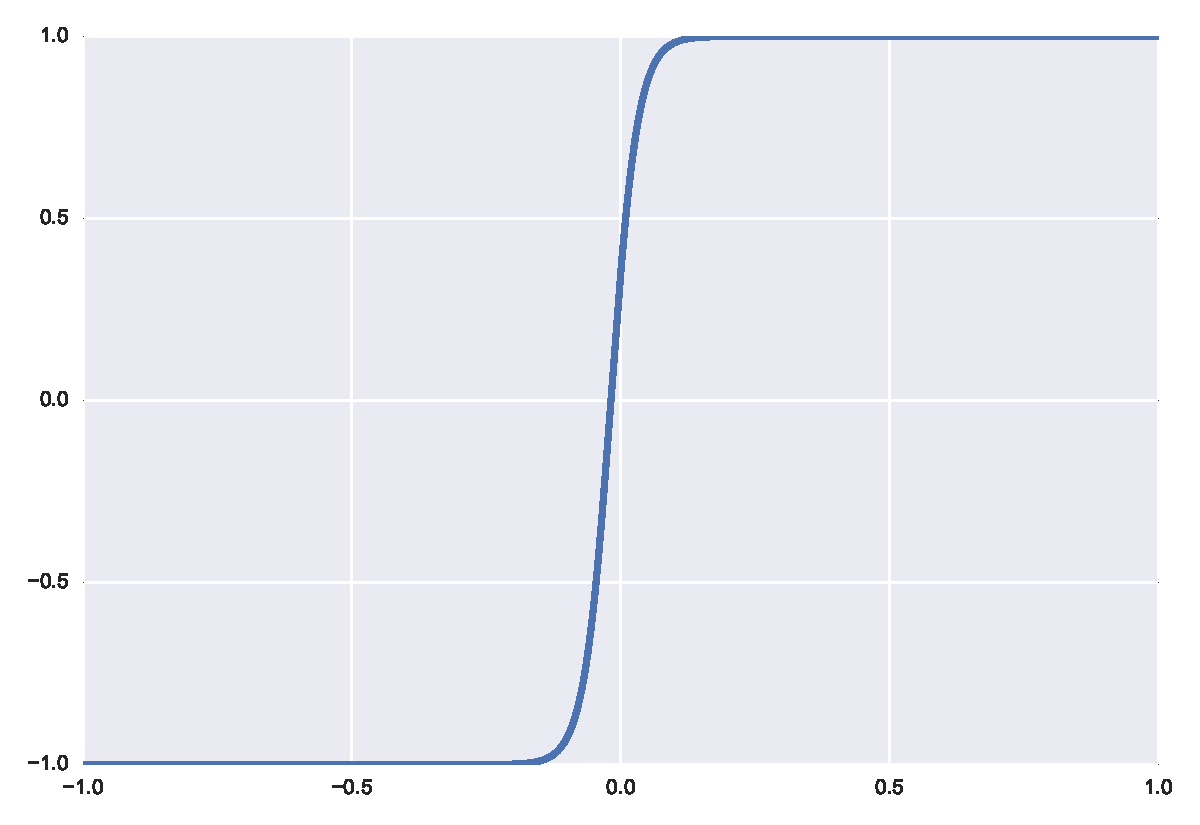
\includegraphics[width=0.7\textwidth]{/Users/dsondak/Documents/Research/Notebook/Research-Notebook/figures/2016/July/burgers_shock.pdf}
  \caption{Illustration of \fenics solution to the steady Burger's equation~\eqref{eq:burgers} using $5000$ finite elements.}
  \label{fig:burgers_shock}
\end{figure}

Next, I need to figure out how to introduce the stabilization parameter into
\fenics.  I'll base this off of Umberto's \fenics implementation of the
stabilization parameter.  Once the stabilization parameter is working, I can 
code up the magnetic field equation, followed by the nondiagonal stabilization
parameter.  Then I will introduce the nondiagonal stabilization parameter and
start compiling the results and the paper.  I will also probably need to
test everything on a two-dimensional problem.  We know that Hartmann flow
doesn't work great.  I'll have to think of another one.

\end{document}
